\subsubsection{UC2 - Login}

\begin{figure}[h!]
	\centering
	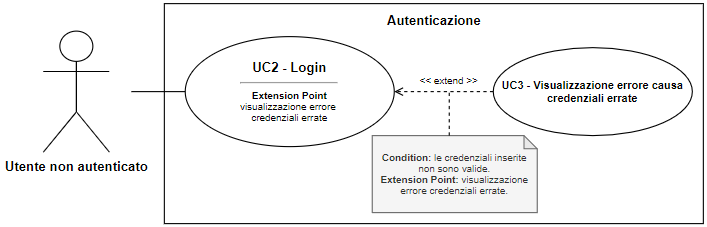
\includegraphics[width=15cm]{images/autenticazione.png}
	\caption{Diagramma Autenticazione}
\end{figure}

\begin{itemize}
	\item \textbf{Attori Primari:} utente non autenticato;
	\item \textbf{Descrizione:} l'utente tenta di autenticarsi usando le sue credenziali;
	\item \textbf{Scenario principale:} l'utente non è ancora autenticato nella piattaforma ed esegue login;
	\item \textbf{Precondizione:} l'utente non è autenticato nella piattaforma;
	\item \textbf{Postcondizione:} l'utente si è autenticato con successo, l'utente viene identificato dal sistema nel ruolo di amministratore o operatore. A seconda del ruolo vengono rese disponibili diverse funzionalità.
	\item \textbf{Estensione:}
		\begin{itemize}
			\item \textbf{UC3}: l'utente visualizza un messaggio d'errore dovuto al fatto che ha inserito delle credenziali errate.
		\end{itemize}
\end{itemize}

\begin{figure}[h!]
	\centering
	\includegraphics[width=9cm]{images/uc2.png}
	\caption{Diagramma UC2 - Login}
\end{figure}

\subsubsection{UC2.1 - Inserimento nome utente}
\begin{itemize}
	\item \textbf{Attori Primari:} utente non autenticato;
	\item \textbf{Descrizione:} al fine di potersi autenticare, l'utente è tenuto ad inserire il suo nome utente, campo obbligatorio;
	\item \textbf{Scenario principale:} l'utente inserisce il suo nome utente;
	\item \textbf{Precondizione:} l'utente non è autenticato nella piattaforma;
	\item \textbf{Postcondizione:} l'utente ha inserito le proprie credenziali.
\end{itemize}	

\subsubsection{UC2.2 - Inserimento password}
\begin{itemize}
	\item \textbf{Attori Primari:} utente non autenticato;
	\item \textbf{Descrizione:} al fine di potersi autenticare, l'utente è tenuto ad inserire la sua password, campo obbligatorio;
	\item \textbf{Scenario principale:} l'utente inserisce la sua password;
	\item \textbf{Precondizione:} l'utente non è autenticato nella piattaforma;
	\item \textbf{Postcondizione:} l'utente ha inserito le proprie credenziali.
\end{itemize}	

\subsubsection{UC3 - Visualizzazione messaggio di credenziali errate}
\begin{itemize}
	\item \textbf{Attori Primari:} utente non autenticato;
	\item \textbf{Descrizione:} l'utente visualizza un messaggio d'errore dovuto al fatto che ha inserito delle credenziali errate;
	\item \textbf{Scenario principale:} l'utente cerca di fare login;
	\item \textbf{Precondizione:} l'utente sta inserendo le proprie credenziali;
	\item \textbf{Postcondizione:} viene visualizzato un messaggio d'errore per notificare l'utente che le credenziali inserite sono errate.
\end{itemize}




